\section{Transition metal dichalcogenides and WS$_2$}
\label{sec:tmd}

In this work we will apply our machine learning-based method
for describing the ZLP to a novel class of tungsten disulfide (WS$_2$) nanostructures~\cite{SabryaWS2}.
%
WS$_2$ is a transition metal dichalcogenide (TMD) material, which 
belongs to a large family of materials known as two-dimensional (2D) materials or Van der Waals materials.
%
In order to interpret  the obtained EEL spectra later in this work, we first need to 
understand the most important characterics of this class of materials.\\

The appreciation for the family of two-dimensional (2D) materials has grown rapidly since the 
first isolation of graphene almost two decades ago~\cite{Novoselov:2004}.
%
Since then, the family of one-atom-thick crystals has grown with the inclusion of metals, semi-conductors
and insulators. 
%
These materials are named two-dimensional to emphasize their extraordinary thinness: 
TMDs are characterised by the remarkable property of being fully 
functional down to a single atomic layer.
%
The properties of these materials are usually very different from their 3D counterparts
and offer great flexibility for tuning their electronic properties on the nanoscale.

Interestingly, numerous possibilities appear when several 2D crystals are combined in one vertical stacking,
allowing for a much greater number of combinations than traditional growth methods.
%
The nature of the intralayer bonds is mostly covalent, whereas the stacking layers 
are held together by weak van der Waals forces, which allows the crystal to easily cleave 
along the layer surface.
%
Such stackings behave signifcantly different from traditional 3D heterostructures, because each layer 
on itself act as both the interface and the bulk material. 
%
This has great influence on the charge displacements: within each layer, charge transfers are reduced
dramatically, however the mobility can be very large between subsequent layers, which offers
interesting possibilities for engineering the band structure.
%
The relative alignment of neighbouring crystals is therefore of great influence on the physics that can be
observed in such crystals.\\


Over the past few years the exploration of these 2D layered materials
 has developed rapidly. 
 %
 In particular significant attention has been 
 going to transition metal dichalcogenides,
 atomically thin semiconductor of the type $MX_2$, here M is a 
transition metal atom (such as Mo or W) and X is a chalcogen atom (such as S, Se, or Te). 
 %
All TMDs have a hexagonal structure,
with each characteristic monolayer comprising one layer of M atoms 
that is sandwiched between two layers of X atoms.
%
As depicted in Fig.~\ref{fig:stackingtypes}, the two most common coordination phases of the monolayers 
are octahedral and trigonal prismatic, which refers to the coordination of the transition metal atom~\cite{Toh:2017}.
%
The electronic properties of TMDs strongly depends on this coordination,
giving rise to a variety of electronic
 and magnetic properties~\cite{Chhowalla:2013}.
 %
As each individual layer can have any of the two coordinations, 
multi-layered TMDs can have a large variety of stacking types (polytypes), 
of which the most commonly found are defined as 1T, 2H and 3R.
%
In this notation, the digit indicates the number of layers in the unit cell and the
letter stands for trigonal, hexagonal and rhombohedral respectively.

Most of the remarkable electronic and optical properties of TMDs
can be traced back to the underlying periodic arrangements of their layers.
%
For example, the 1T form displays metallic behaviour, 
while both 2H and 3R forms are semiconducting.
%
While nanostructures built upon 2H or 3R crystalline phases have been routinely studied,
knowledge about those based on mixed 2H/3R polytypes is far more limited~\cite{SabryaWS2}.

%%%%%%%%%%%%%%%%%%%%%%%%%%%%%%%%%%%%%%%%%%%%%%%%%%%%%%%%%%%%%%%%%%%%%%%%%%%%%%%
\begin{figure}[H]
    \centering
    \includegraphics[width=0.75\textwidth]{plots/stackings.pdf}
    \caption{The most common coordinations and polytypes of TMD unit cells. 
    %
    Stacking single layers with the  octahedral coordination yields a tetragonal symmetry (1T). 
    %
    The prismatic coordination can yield different stacking symmetries: 
    hexagonal (2H) and rhombohedral (3R).
    %
    Retrieved from~\cite{Toh:2017}}.
    \label{fig:stackingtypes}
\end{figure}
%%%%%%%%%%%%%%%%%%%%%%%%%%%%%%%%%%%%%%%%%%%%%%%%%%%%%%%%%%%%%%%%%%%%%%%%%%%%%%%%%%5


Apart from the dependence on the stacking sequence, 
the properties of this class of materials vary significantly
with their thickness. For instance, MoS$_2$ exhibits an indirect bandgap
in the bulk form which becomes direct at the monolayer level~\cite{Splendiani:2010}.
%
The indirect-to-direct bandgap transition is the main reason for the interest in 
the use of TMDs for flexible electronics: it emphasizes the importance of the
mechanical properties of these materials. 
%
However, it tends to be much more difficult to uniformly deform 2D monolayers
of a material compared to bulk samples, and therefore measuring on 2D systems
can be challenging.
%
TMDs are often combined with other 2D materials like graphene
to make Van der Waals heterostructures, which need to be tuned in order
to function as building blocks for many devices such as LEDs, solar cells, 
transistors, and photodetectors.
%
This research field is still emerging and highly promosing to have a big
impact on future nanotechnology. \\
 
An example of a TMD exhibiting a pronounced dependence on its thickness is 
thungsten disulfide (WS$_2$), with an indirect-to-direct bandgap transition when going
from bulk to bilayer or monolayer form.
%
The effects of this transition are manifested as enhanced
photoluminescence in monolayer WS$_2$, whereas only little emission is observed in
the corresponding bulk form.
%
WS$_2$ adopts a layered structure by stacking atomic layers of S-W-S 
in a sandwich-like configuration, with each monolayer of the trigonal prismatic type (Fig.~\ref{fig:stackingtypes}). 
%
Although the interaction between adjacent layers is a weak Van der Waals 
force, the dependence of the interlayer interaction on the stacking 
order of WS$_2$ is significant.
%
Further applications of this material include storage of hydrogen 
and lithium for batteries~\cite{Bhandavat:2012}.

%%%%%%%%%%%%%%%%%%%%%%%%%%%%%%%%%%%%%%%%%%%%%%%%%%%%%%%%%%%%%%%%%%%%%%%%%%%%%%%
\begin{figure}[h]
    \centering
    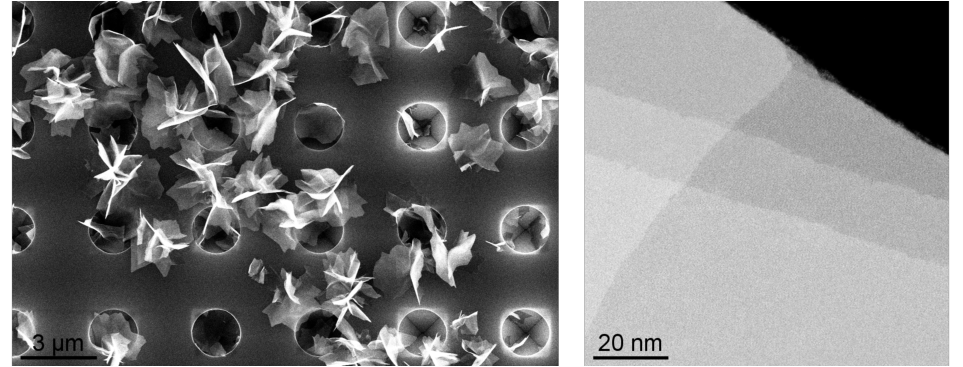
\includegraphics[width=0.8\textwidth]{plots/spectrumimage.pdf}
    \caption{Left: low-magnification TEM image of WS$_2$ nanoflowers
      grown on top of a porous TEM substrate. Right: the magnification of a representative 
      petal of a nanoflower, where the black region corresponds to 
      the vacuum (no substrate) and the difference in contrast indicates terraces of varying thickness.}
    \label{fig:nanoflowers}
\end{figure}
%%%%%%%%%%%%%%%%%%%%%%%%%%%%%%%%%%%%%%%%%%%%%%%%%%%%%%%%%%%%%%%%%%%%%%%%%%%%%%%%%%5

For this work, we have studied specific nanostructures of WS$_2$ called nanoflowers,
which are presented in~\cite{SabryaWS2}. 
%
A low-magnification TEM image of the WS$_2$ nanoflowers is displayed
in the left panel of Fig.~\ref{fig:nanoflowers}.
%
These structures are grown directly on top of a TEM substrate with holes in it. 
%
The right panel shows the magnification of a representative petal of a nanoflower,
where the difference in contrast indicates terraces of varying thickness.
%
Note that the black region corresponds to the vacuum, without
substrate underneath.
%
These WS$_2$ nanoflowers contain areas with different thicknesses, orientations
and crystalline structures, therefore representing an ideal environment to investigate
structural morphology in WS$_2$ with electronic properties at the nanoscale.

What makes it even more interesting is that these nanoflowers exhibit a mixed form of 3R/2H polytypism, 
which is of importance for the interlayer interactions: 
it has been observed that the coexistence of multiple stacking types can complicate
the characterization of the physical properties~\cite{Na:2018}.
%
For example, one possible response of polytypism to electric fields is
 spontaneous electrical polarization, leading to modifications on the 
 electronic band structure and correspondingly on the band gap~\cite{Li:2016}.
 %
Tailoring the specific stacking sequences
represents a powerful strategy to identify and design novel physical properties~\cite{SabryaWS2}.\\

As mentioned before, one of the most interesting properties of TMDs that also
occurs in WS$_2$ is the fact when the material
is thinned down to a single monolayer, its indirect band gap of
$E_{\rm bg}\simeq 1.4$ eV
switches to a direct band gap of approximately $E_{\rm bg}\simeq 2.1$ eV.
%
In general, it has been found that the type and magnitude of the bandgap
of WS$_2$ depends quite sensitively on the crystalline structure and
the number of layers that constitute the material.
%
In Table~\ref{table:bgvalues} we collect
representative results for the determination of the bandgap energy $E_{\rm bg}$
and its type in WS$_2$, obtained by means of different experimental and theoretical techniques.
%
For each reference we indicate separately the bulk results and those
obtained at the monolayer level.
%
We observe that for monolayers, the results for the measured
value of $E_{\rm bg}$ are quite inconsistent, 
reflecting the challenges of its accurate determination.

 
%%%%%%%%%%%%%%%%%%%%%%%%%%%%%%%%%%%%%%%%%%%%%%%%%%%%%%%%%%%%%%%%%%%%%%%%%%%%%%%%%%%%%
\begin{table}[H]
  \small
  \begin{centering}
   \renewcommand{\arraystretch}{1.20}
\begin{tabular}{ccccc}
\br
Reference                       & Thickness & $E_{\rm bg}$ (eV)  & Band gap type  & Technique \\
\mr
{\cite{Braga:2012}} & bulk   & $1.4\pm0.07$            & indirect  & {Gate-voltage dependence}  \\
\mr
\multirow{}{}{\cite{Jo:2014}}                 & ML   & $2.14 $         & direct  & \multirow{}{}{Gate-voltage dependence}        \\
& bulk & $1.40 $    & indirect              \\
\mr

\multirow{}{}{\cite{Gusakova:2007}} & ML   & $2.03\pm0.03$            & direct  & \multirow{}{}{DFT}  \\
& bulk & $1.32\pm0.03 $            & indirect     \\
\mr
\multirow{}{}{\cite{Kam:1982}}                  & ML   & $1.76\pm0.03 $      & direct    & \multirow{}{}{Absorption edge coefficient fitting}         \\
& bulk & $1.35 $          & indirect        \\
\mr
\cite{Shi:2013}                & ML   & $2.21\pm0.3 $         & direct  & Bethe-Salpeter equation (BSE)        \\                 \br                                         
\end{tabular}
\vspace{0.27cm}
\caption{Representative results for the determination of the bandgap energy $E_{\rm bg}$
  and its type in WS$_2$, obtained from a variety of experimental and theoretical techniques.
  %
  For each reference we indicate separately the bulk results and those
  obtained for a monolayers}
    \label{table:bgvalues}
    \end{centering}
\end{table}
%%%%%%%%%%%%%%%%%%%%%%%%%%%%%%%%%%%%%%%%%%%%%%%%%%%%%%%%%%%%%%%%%%%%%%%%%%%%%%%%%%%%%%
